\documentclass{article}
\usepackage{tikz}
\usetikzlibrary{arrows.meta}

\begin{document}

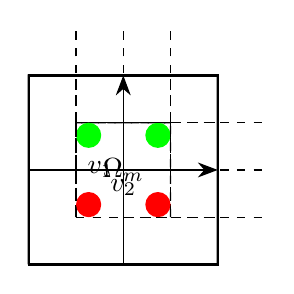
\begin{tikzpicture}[scale=0.8]
    % Define the coordinates for the vertices of the cube
    \def\cubeSize{3}
    \coordinate (A) at (-\cubeSize/2,-\cubeSize/2);
    \coordinate (B) at (\cubeSize/2,-\cubeSize/2);
    \coordinate (C) at (\cubeSize/2,\cubeSize/2);
    \coordinate (D) at (-\cubeSize/2,\cubeSize/2);
    
    % Draw the cube
    \draw[thick] (A) -- (B) -- (C) -- (D) -- cycle;
    \draw[thick] (A) -- ++(0,\cubeSize) -- (C);
    \draw[thick] (B) -- ++(0,\cubeSize) -- (D);
    
    % Define the coordinates for the subdomains
    \def\subdomainSize{1.5}
    \coordinate (A1) at (-\subdomainSize/2,-\subdomainSize/2);
    \coordinate (B1) at (\subdomainSize/2,-\subdomainSize/2);
    \coordinate (C1) at (\subdomainSize/2,\subdomainSize/2);
    \coordinate (D1) at (-\subdomainSize/2,\subdomainSize/2);
    
    % Draw the subdomains
    \draw[dashed] (A1) -- (B1) -- (C1) -- (D1) -- cycle;
    \draw[dashed] (A1) -- ++(0,\subdomainSize) -- (C1);
    \draw[dashed] (B1) -- ++(0,\subdomainSize) -- (D1);
    
    % Define the coordinates for the particles
    \def\particleSize{0.2}
    \coordinate (z11) at (-\subdomainSize/2+\particleSize,-\subdomainSize/2+\particleSize);
    \coordinate (z12) at (-\subdomainSize/2+\particleSize,\subdomainSize/2-\particleSize);
    \coordinate (z21) at (\subdomainSize/2-\particleSize,-\subdomainSize/2+\particleSize);
    \coordinate (z22) at (\subdomainSize/2-\particleSize,\subdomainSize/2-\particleSize);
    
    % Draw the particles
    \fill[red] (z11) circle (\particleSize);
    \fill[green] (z12) circle (\particleSize);
    \fill[red] (z21) circle (\particleSize);
    \fill[green] (z22) circle (\particleSize);
    
    % Draw the vectors
    \draw[-{Stealth[scale=1.5]}] (0,-\cubeSize/2) -- node[left] {$v_1$} (0,\cubeSize/2);
    \draw[-{Stealth[scale=1.5]}] (-\cubeSize/2,0) -- node[below] {$v_2$} (\cubeSize/2,0);
    
    % Label the subdomain
    \node at (0,0) {$\Omega_m$};
    
    % Draw the dashed lines for the subdomains
    \foreach \x in {-1,0,1} {
        \foreach \y in {-1,0,1} {
            \draw[dashed] (\x*\subdomainSize/2,\y*\subdomainSize/2) -- ++(\subdomainSize,0);
            \draw[dashed] (\x*\subdomainSize/2,\y*\subdomainSize/2) -- ++(0,\subdomainSize);
        }
    }
\end{tikzpicture}

\end{document}